% ProjectD

\chapter{Project Description}

\label{ProjectD}

\lhead{Chapter 5. \emph{Project Description}}

%----------------------------------------------------------------------------------------
%	Ara platform discovery
%----------------------------------------------------------------------------------------

\section{Ara platform study}

In this section, we will describe different studies and preliminary experimentation we've done before designing  the module.

In fact, because of the lake of literature or past experience with the Ara platform, we first need to study the Ara Module Development Kit send by Google ATAP. We focus on understanding the role of each board, and there I/O - regarding protocols and speed. Then we determine the reliable rate on witch the operating system can execute a single task - such as I/O operation. Finally we perform some benchmark and CPU load test. 

\subsection{MDK and boards study}

\subsection{Android for ARA reliable I/O operation rate}  \label{result-ara}

\subsubsection{Problematic}

In this part, we would determine the I/O performance between the Ara main board and  modules in order to fit its characteristics: maximum ADC sampling rate, resolution, buffering needs.

We focused on the minimum stable thread execution speed, which fix the number of Android I/O operation per second, then the maximum number of bytes we can read each time.

\subsubsection{Protocol}
We modify the oxymeter application changing the thread execution interval from 1ms to 100ms and record the effective execution period using time-stamps. To have a set consistent datasets, we record 1 million of sample for each measure. As consequence, we would be able to determine the minimum thread execution period, and its stability.
This point is particularly important for designing the buffer on the VLC receiver : a bigger I/O operation period than expected will cause overflow, and data loss of data.

To determine the bus speed and the max effective transferred without error for each operation, we replaced the oxymeter module by an Arduino that will write different among of data on the bus. In addition, we use a logic analyzer to record what's happening on the bus.

\subsubsection{Results}

\begin{figure}[h]
  \begin{minipage}[c]{.46\linewidth}
    \centering
 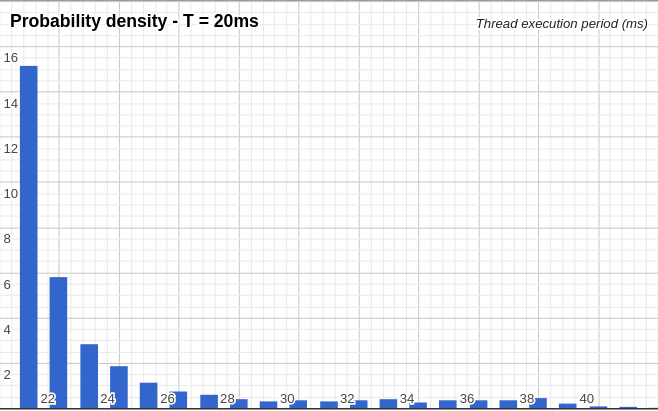
\includegraphics[width=\textwidth, height=.70\linewidth]{Pictures/dsp20.png}
    \label{fig:dsp20}
    \rule{16em}{0.5pt}
    \caption[Probability density of Android thread execution interval with 20ms as defined period]{Probability density of Android thread execution interval with 20ms as defined period}
  \end{minipage}
  \hfill%
  \begin{minipage}[c]{.46\linewidth}
  \centering{
    \scalebox{1}{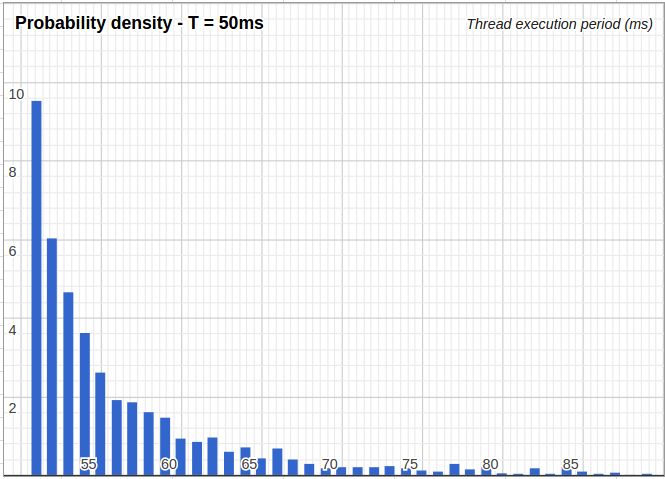
\includegraphics[width=\textwidth]{Pictures/dsp50.png}}}
    \label{fig:dsp50}
    \rule{16em}{0.5pt}
    \caption[Probability density of Android thread execution interval with 50ms as defined period]{Probability density of Android thread execution interval with 50ms as defined period}
  \end{minipage}
  
\end{figure}
\begin{center}
Remark : as value lower than expected have no consequences, we doesn't plot them on the chart, but are taken in account in the probability repartitions.
\end{center}

\begin{itemize}
\item Android threads can't reach lower period than 8ms but with an elevate variance, as we can see in .

\item Performing statistical analysis, for each execution period and plotting the effective period distribution and variance, we can consider 30ms as safe.

\item Even if the I2C bus speed clock should be 400kHz - according to the Ara MDK documentation - the effective clock rate is 133kHz.
On other hand, even if the kernel driver limits I/O operations to 512 bytes, the bus gets corrupted trying to transfer more than 350 bytes per operation.
\end{itemize}

\subsubsection{Conclusion}  \label{conclusion-ara}
According to \ref{result-ara}, we should design our VLC receiver module to taking account an effective bit-rate of 92,4 kbps and will developed the Android application with a module polling thread period to 30ms and an I2C transaction . 


\subsection{Ara benchmark}

In addition to \ref{result-ara}, we should be sure that a normal to extensive modular smartphone won't affect VLC module performances, even if the app run in background mode. In this case, the Android CPU governor will reduce the priority of our app, giving it less resources or stopping it if necessary.

In order to do that, we use a benchmark application that would simulate typical smartphone use-case : web browsing, shot-message writing, video playing or games.

During the stress tests, both CPU load and repartitions over running process, and RAM usage are monitored.

\begin{figure}[htbp]
    \centering{
    \scalebox{0.5}{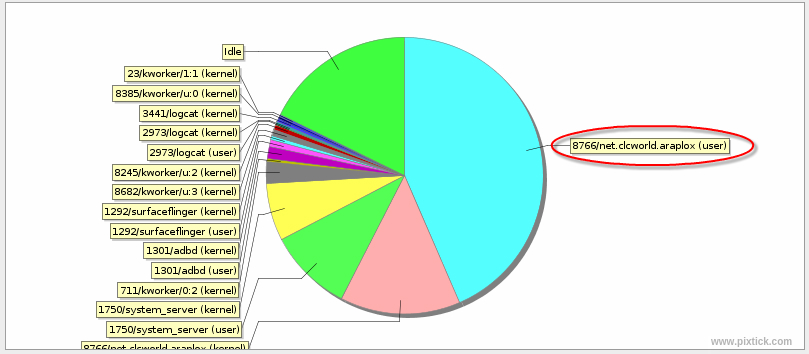
\includegraphics[width=\textwidth]{Pictures/cpu-singleapp.jpg}}}
    \label{fig:cpu-single}
    \rule{35em}{0.5pt}
    \caption[CPU load and repartitions with only Oxymeter application running]{CPU load and repartitions with only Oxymeter application running}
\end{figure}


\begin{figure}[htbp]
    \centering{
    \scalebox{0.5}{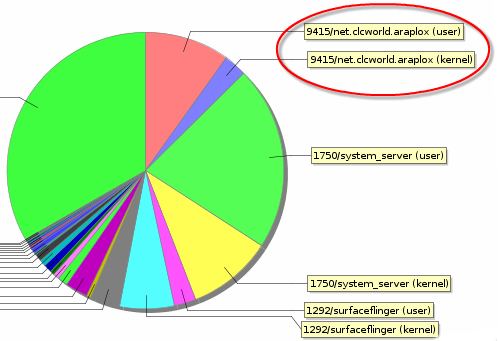
\includegraphics[width=\textwidth]{Pictures/cpu-loadapp.jpg}}}
    \label{fig:cpu-load}
    \rule{35em}{0.5pt}
    \caption[CPU load and repartitions during the web navigation simulation]{CPU load and repartitions during the web navigation simulation}
\end{figure}

For each case, except the video game that made freeze and crash the Ara platform, results where exactly the same than with a single activity - ie. just our application - and we achieve the same bit-rate.

\subsubsection{Conclusion}
{
Following conclusion in\ref{result-ara}, we are now able to determine the Digital-to-Analogic converter characteristic. In order to get the better ratio as possible between the resolution, the sampling rating, and and the clock rate we can achieve with the LED Driver Emitter,chosen values are summarized in the next table.

\begin{table}[htbp]
\begin{center}
\begin{tabular}{|l|c|r|}
  \hline
  Sampling Rate & $\approx$ 1 MSPS \\
  \hline
  Resolution & 8-12 bits \\
  \hline
  Buffer Size & 200 bytes\\
  \hline
\end{tabular}
\end{center}
\caption{DAC needs summary}
\label{tab:conclusion-adc}
\end{table}
}

%----------------------------------------------------------------------------------------
%	Receiver circuit design
%----------------------------------------------------------------------------------------

\section{Receiver circuit design}

In this section, we will focus on the VLC module hardware design, that will have a major impact in the quality and efficiency of our system. Main difficulty we have to face here, is to select appropriate circuit pattern, filters type and cute-off frequency, according to the channel characteristic. The method we applied was in a first to study the channel principal characteristic, to design a first circuit, then compute theoretical values, and finally adjust them after some practical results. 

\subsection{Needs description}

The VLC receiver front-end circuit must detect with high frequency precision the modulated light within a range starting from 1kHz to 1Mhz. Before digitalization, the current generated by the photodiode has to be converted into current.
As a major issue in VLC are interferences - from the ambient light or UV from the sun - the signal should be properly filtered and amplified before digitalization.

Our solution is constituted with a photodiode, witch convert the modulate light into current. It's followed by a trans-impedance amplifier in order to convert the photodiode output current into tension. Then, an analogical low-pass filter and gain are applied, before digitalization by the a micro-controller unit.

\subsection{1st AOP : Current to tension converter}

\begin{figure}[htbp]
    \centering
    \scalebox{0.4}{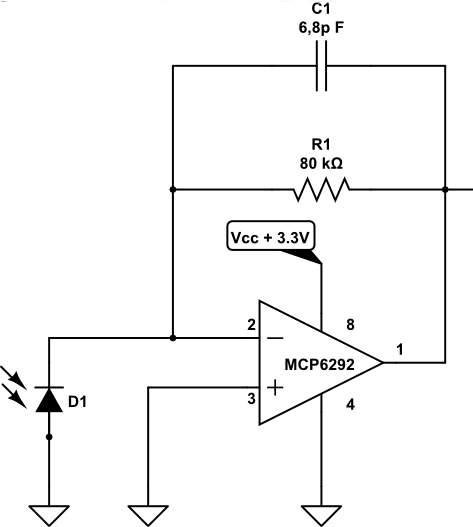
\includegraphics[width=\textwidth]{Pictures/TIA.png}}
    \rule{35em}{0.5pt}    
    \caption{Trans-Impedance Amplifier}
    \label{fig:tia}
\end{figure}

The first part of the circuit is the Trans-Impedance Amplifier, presented in \ref{fig:tia}. TIA is a standard electronic pattern made from an operational amplifier and a resistor to convert the current to a tension.

We choose the MCP6292 Op-Amp for its 10MHz wide band pass, and 3.3V input voltage. Indeed, the interesting input frequency  from modulated light won't be greater than 1MHz and we will be able supply it with the MCU.
The DC output voltage due to the photodiode is given by \ref{eq:vout} 

\begin{equation}
V_{OUT}  = I_{DI} * R_{1}
\label{eq:vout}
\end{equation}

The capacitance in the feed-back loop is determined to compensate the photodiode capacitance in order to assure the operational amplifier stability which depends on $C_1$, $R_1$ and $C_{D1}$.

\subsection{2nd: High Pass filter}

After the Trans-Impedance Amplifier circuit part, we add a high-pass (figure \ref{fig:hpf} filter to attenuate the noise from the ambient lights such as sunlight and 50-60kHz indoor fluorescent lights.

To perform, the filter was designed with a cut-off frequency of 200Hz. We chose $C3$ and $R2$ value. According to figure \ref{fig:hpf-bode} and equation \ref{eq:ht-fc}, we use 10nF capacitance and 48kH$\Omega$ resistor
\begin{equation}
f_{cf}  = \frac{1}{2\pi RC}
\label{eq:ht-fc}
\end{equation}

\begin{figure}[htbp]
    \centering
    \scalebox{0.3}{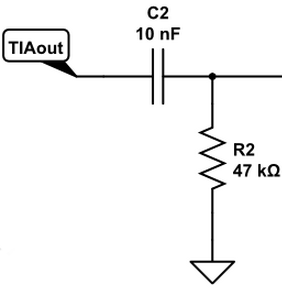
\includegraphics[width=\textwidth]{Pictures/HF-Filter.png}}
    \rule{35em}{0.5pt}
    \caption{High-Pass Filter}
    \label{fig:hpf}
\end{figure}

\begin{figure}[htbp]
    \centering
    \scalebox{0.7}{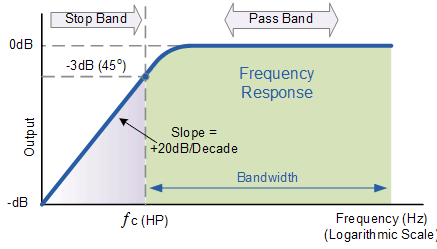
\includegraphics[width=\textwidth]{Pictures/hpfilter.png}}
    \rule{35em}{0.5pt}
    \caption{High-Pass Filter Bode Plot}
    \label{fig:hpf-bode}
\end{figure}
\subsection{Gain}


The output gain in the second part of the circuit aims to increase the signal amplitude, without increasing the noise. As a result, we will get better $SNR$, and digital signal processing and thresholding will be more accurate.

As for the TIA, a capacitance $C_3$ of $6.8pF$ has been added to assure the AOP stability.

The gain $G_{OUT}$ has been adjusted during our final experiments with the modulated LED and its value is given by \ref{eq:gain}

\begin{equation}
G_{OUT}  = \frac{R_{4}}{R_{5}}
\label{eq:gain}
\end{equation}


\begin{figure}[htbp]
    \centering
    \scalebox{0.3}{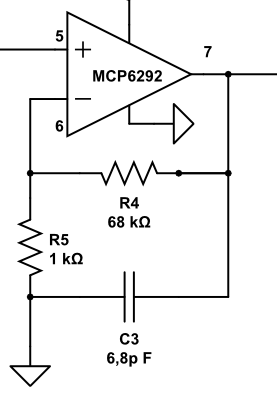
\includegraphics[width=\textwidth]{Pictures/LPFilter.png}}
    \rule{35em}{0.5pt}
    \caption{Gain Operational Amplifier}
    \label{fig:lpf}
\end{figure}

%----------------------------------------------------------------------------------------
%	Emitter driver
%----------------------------------------------------------------------------------------

\section{Emitter driver}

In this section, we will discuss the LED emitter and driver we developed for our system.
 
A commercial LED has been used as a modulated light source with an on-off signal generated by a micro-controller unit, that carry transmitted data encoded using a modified 4B6B run-length limited coding.

\subsection{hardware}
The MCU used as LED Driver is an STM32L0, exactly the same as for the receiver, as its development kit is low cost, and toolchains, and software development environment can be shared. We exploited its 3.3V digital output to blink the emitter white LED.

\subsection{OOK modulation}
Following IEEE 802.15.7 recommendations, we propose to use an On-Off Keying modulated signal as described in \ref{ook} meaning that each bit 1 is mapped onto an high output level, and bit 0 mapped onto null output on the digital micro-controller output. 

\subsection{4B6B Line coding}

The line code used is a modified version of the standard 4B6 described in \ref{rll} to increase the transmitted power.
4 bits are mapped into 6bits always using 4 bit 1 and 2 bit 0. In that way, duty cycle is 2/3 instead of 1/2 for the standard version. This modified version would be used as error detection too.

\begin{table}[htbp]
\begin{center}
\begin{tabular}{|l|c|r|}
  \hline
  4 bits & 6 bits \\
  \hline
  0000 & 001111 \\
  0001 & 010111 \\
  0010 & 011011 \\
  0011 & 011110 \\
  0100 & 011110 \\
  0101 & 100111 \\
  0110 & 101011 \\
  0111 & 101101 \\
  1000 & 101110 \\
  1001 & 101111 \\
  1010 & 110011 \\
  1011 & 110101 \\
  1100 & 110110 \\
  1101 & 111001 \\
  1110 & 111010 \\
  1111 & 111100 \\
  \hline
\end{tabular}
\end{center}
\caption{Modified 4B6B}
\label{tab:m4b6b}
\end{table}


To compare the performance between different RLL coding, Manchester has been implemented to, and both coding schema can be easily switched programmatically using a C macro.

\subsection{Transmission Pattern} \label{frame}

We propose a transmission pattern that would easly permit clock synchronization on the receiver. In addition, it has been designed taking account of the flickering and dimming issue.

Three transmissions state are defined : 
\begin{itemize}
\item Idle : no data are transmitted, but we keep transmitting continuously \textbf{111000} and \textbf{000111} 4B6B symbols.
\item Preamble : just before sending the data, the emitter should send a preamble, to let the receiver synchronizing. Symbols used should be different than these used to encode the data. We propose a combination of \textbf{110100} and \textbf{001011}.
\item Data : 4B6B encoded data.

The table \ref{tab:trans2} shows the transmission of the number 2, 16 bits encoded : 0000 0000 0000 0010.

\begin{table}[htbp]
\begin{center}
\makebox[\textwidth][c]{\begin{tabular}{|c|c|c|c|}
  \hline
  Idle & Preamble & Data & Idle \\
  \hline
  000111 111000 000111 & 110100 001011 & 001111 001111 001111 011011 & 000111 111000 000111 \\
  \hline
\end{tabular}}
\end{center}
\caption{A transmission example : 2 (16-bits)}
\label{tab:trans2}
\end{table}


\end{itemize}
\subsection{Algorithm}





%----------------------------------------------------------------------------------------
%	Receiver ADC and Buffer
%----------------------------------------------------------------------------------------

\section{Receiver ADC and Buffer}
In this section, we will describe the digitalization and digital processing performed by the VLC receiver module, just  after the front-end circuit.

\subsection{Hardware choice}

According to \ref{tab:conclusion-adc}, we chose to use the STM32L0 micro-controller based on an ARM Cortex  M0+ processor with these characteristics :
\begin{itemize}
\item Processor Frequency up to 32 MHz: it will let us embedded some signal processing in order to reduce the computation on the Android.
\item Low power consumption : 87 $\mu$A/MHz: it's a key feature for the mobile battery harvesting.
\item Analogical Input with 1.1 MSPS ADC : it fits our requirements.
\item Different I/O, including I2C : it's a requirement to connect the MCU to the MDK endpoint board.
\item 8kB RAM : this feature will let us implements the buffering using software memory.
\end{itemize}

\subsection{Software implementation}

We developed the MCU software in C, using the Arm GCC tool-chain and ST-Link debugger interface included in the Em::Blocks \citep{emblocks} IDE.

The MCU is initialized setting the HSI as source clock with 32MHZ as processor frequency. Only I$^2$C, UART, ADC are enabled.

The main program works in interrupt mode. 

\subsubsection{Data Acquisition}

The ADC sampling rate is set to 1,1 MSPS, in order to get the higher frequency precision, and the resolution to 8 bits, sufficient for OOK modulation.

The acquisition is done using buffering and Direct Memory Access (DMA) mode. 
When the DMA buffer is full, an interruption is thrown starting the demodulation and RLL decoding process.

\subsubsection{Demodulation and RLL Decoding}

First step is the the OOK demodulation that consisting in applying a threshold to the value.

\lstinputlisting[language=C, caption=Thresholding implementation ,label=Thresholding, firstline=159, lastline=163]{CodeReceiver/adc.c}

As explain in \ref{frame}, we should detect the preamble pattern - 00011000000 - that would help synchronize both emitter and receiver.
Then as we know exactly the data frame and structure, we would be able to read the 4B6B encoded data.


\subsubsection{Buffering}


After being decoded , bits are pushed into a FIFO Buffer implemented in \ref{fifo.c}

\lstinputlisting[language=C, caption=fifo.c ,label=DescriptiveLabel, firstline=37, lastline=45]{CodeReceiver/main.c}

\subsubsection{Input/output}
 
\begin{enumerate}
\item UART peripheral is enabled only when debugging or saving measure to the laptop via Serial->USB port.

\item I$^2$c is enabled in slave mode and connected to the Ara module development board. An interruption is thrown when a read request is detected from the master peripheral driven by the Android application.

The function called in the interruption callback get last 
\end{enumerate}

%----------------------------------------------------------------------------------------
%	Ara Android App
%----------------------------------------------------------------------------------------

\section{Ara Android App}

In this part, we describe the Android application that we have developed, to support our VLC receiver module.

\subsection{Application structure and operations}
Our application as been developed used Google Android API 18, to be compliant with the operating system version which has been installed on the AP Board.

The application package has been called respecting Java name convention : edu.upc.entel.wng.vlcAraModule and content 3 classes :

\begin{itemize}
\item VLCAraActivity : initialize the application and user interface. It surcharges the Activity class , as requested by the Android API.
\item Sensor : define and perform operations to communicate with our module such as I2C bus initialization, data polling as well as handling and message with the User Interface (UI).
\item VlcLogger : this class realize logging operation saving received data on the board internal storage or an external SD Card.
\end{itemize}

Application workflow is quiet simple :
\begin{enumerate}
\item Initialize and start the application main Activity.
\item Setup the I2C Bus.
\item Initialize the logger and create a log file.
\item Start the \textbf{Sensor} thread that poll I2C bus at defined interval and send the result to the android activity. 
\item Handle Sensor thread messaging and user interaction.
\end{enumerate}

\subsection{User Interface}

The application user interface as few components as defined in the XML activity layout description file :
\begin{itemize}
\item EditText field: used to display received bits.
\item "Clear" and "Save" Button :
\end{itemize}

Each component are placed in a horizontal layout container.

\begin{figure}[htbp]
    \centering
    \scalebox{0.6}{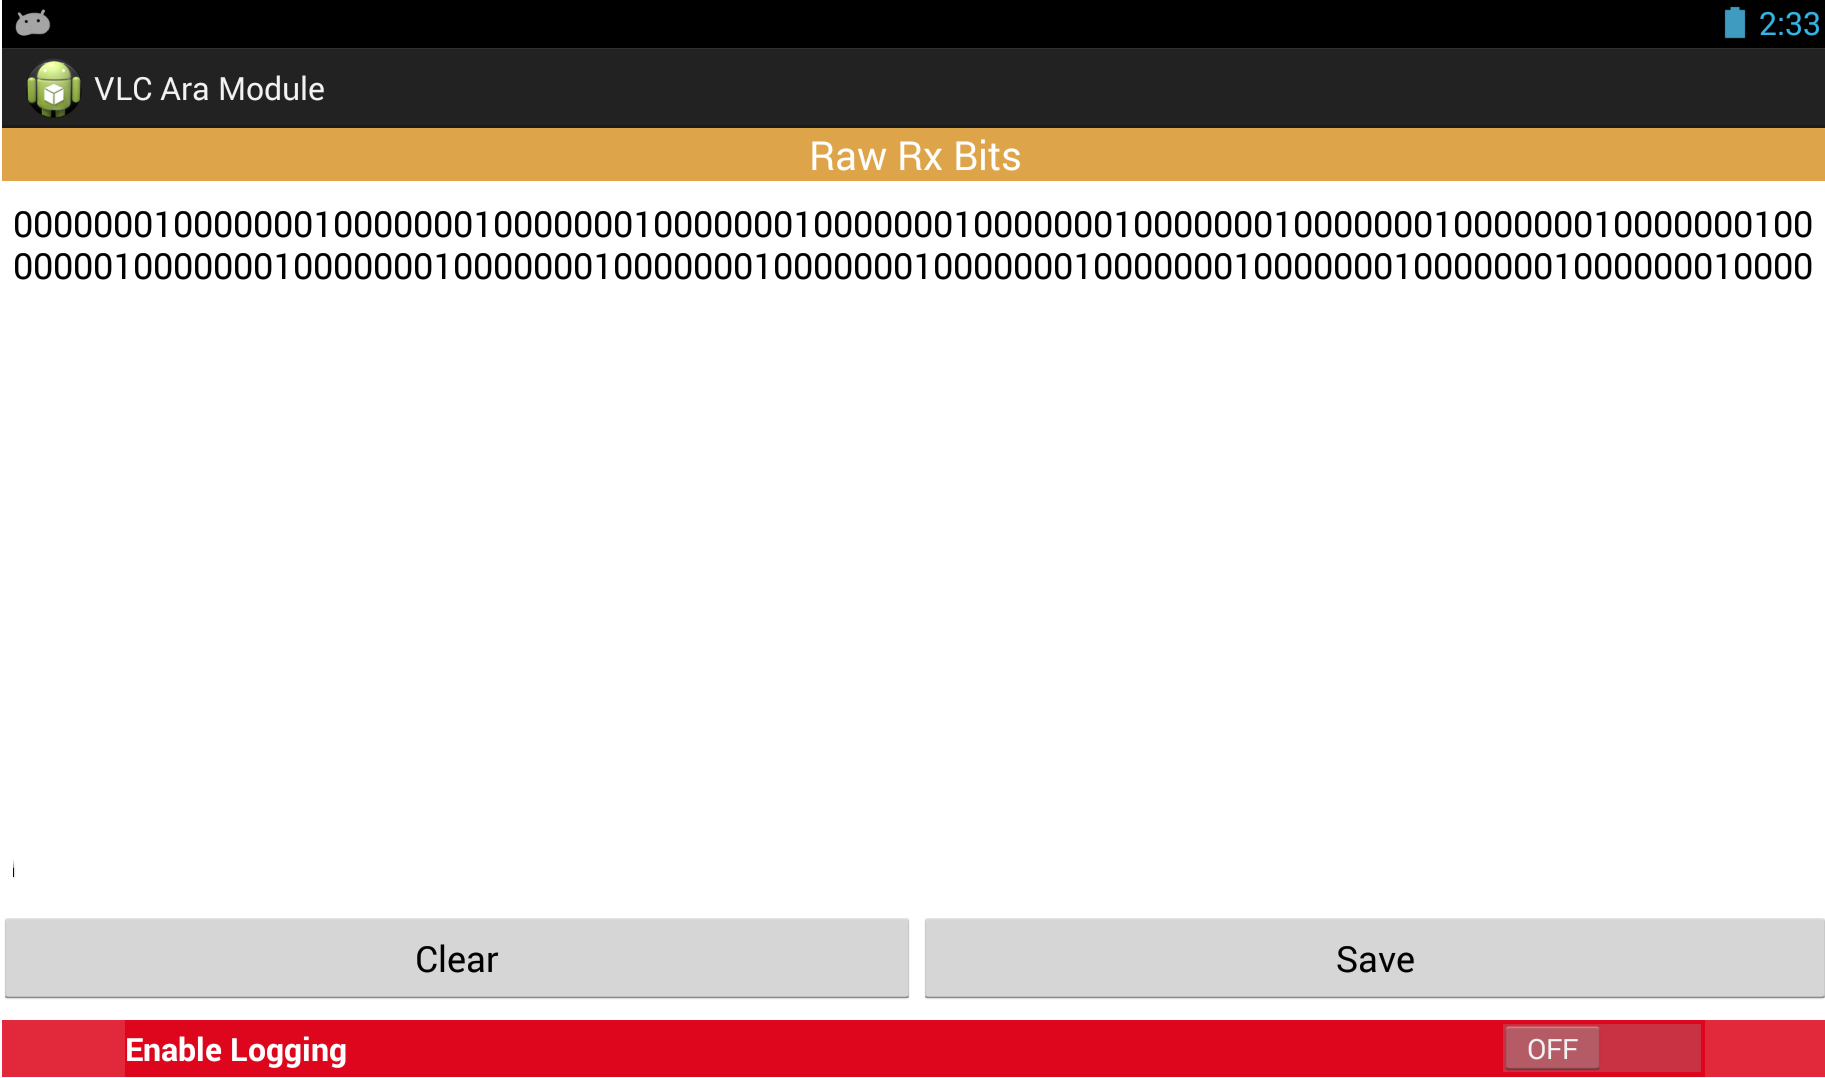
\includegraphics[width=\textwidth]{Pictures/android.png}}
    \rule{35em}{0.5pt}
    \caption{Android application receiving data via VLC}
    \label{fig:androidapp}
\end{figure}

\subsection{I2C JNI interface}

As the Android Java API for the Ara Module Development Kit is the same as the standard API, we need to implement additional components in order to access the low level hardware such as the GPIO or the I2C bus.
The Ara MDK is provided with an operating system level driver, developed in C, that can be used to configure, read and write date, in a simple way.
However, this C interface, can't be directly used through the Java API. In order to give the possibility to perform I2C operations in our Android application, we develop a JNI interface that would wrap the C driver into a Java package.
So we define 2 Java classes : 
\begin{itemize}
\item I2CManager : it configures the i2c bus, by using UNIX I2C kernel driver and execute operations defined in I2CTransaction.
\item I2CTransaction : it represents read or write operation on the bus.
\end{itemize}

Class methods are detailed in the \citep{an:e}.
